% Gemini theme
% See: https://rev.cs.uchicago.edu/k4rtik/gemini-uccs
% A fork of https://github.com/anishathalye/gemini

\documentclass[final]{beamer}

% ====================
% Packages
% ====================
\usepackage{amsfonts}
\usepackage[T1]{fontenc}
\usepackage{lmodern}
\usepackage[size=custom,width=30,height=48,scale=1.0]{beamerposter}
\geometry{paperwidth=30in,paperheight=48in}
\usetheme{gemini}
\usecolortheme{ucf}
\usepackage{graphicx}
\usepackage{booktabs}
\usepackage{tikz}
\usepackage{pgfplots}
\pgfplotsset{compat=1.17}

% ====================
% Lengths
% ====================

% If you have N columns, choose \sepwidth and \colwidth such that
% (N+1)*\sepwidth + N*\colwidth = \paperwidth
\newlength{\sepwidth}
\newlength{\colwidth}
\setlength{\sepwidth}{0.025\paperwidth}
\setlength{\colwidth}{0.3\paperwidth}

\newcommand{\separatorcolumn}{\begin{column}{\sepwidth}\end{column}}

% ====================
% Title
% ====================

\title{\textbf{Research Funded Project}\\
``Rapid  and Accurate  INS Transfer Alignment \\ for Air  Launched Tactical Missile\\ Using  Kalman  Filter''}

\author{Dr. Tapan  Kumar  Jain}

\institute[IIITN]{\textit{Indian Institute of Information Technology, Nagpur}}

% ====================
% Footer (optional)
% ====================


\footercontent{
  \href{https://iiitn.ac.in}{https://iiitn.ac.in} \hfill
  PhD Cell, IIIT Nagpur, August 2023 \hfill
  \href{mailto:skjain.drdl@gov.in}{skjain.drdl@gov.in}}
\begin{document}
\addtobeamertemplate{headline}{}
{
    \begin{tikzpicture}[remember picture,overlay]
      \node [anchor=north west, inner sep=3cm] at ([xshift=0.0cm,yshift=3cm]current page.north west)
      {
\includegraphics[height=12cm]{logos/ucf_logo2.png}}; % also try shield-white.eps
      \node [anchor=north east, inner sep=3cm] at ([xshift=1.0cm,yshift=3cm]current page.north east)
 {
\includegraphics[height=12cm]{logos/DRDO1.jpeg}};
    \end{tikzpicture}
}

\begin{frame}[t]
\begin{columns}[t]
\separatorcolumn

\begin{column}{\colwidth}

  \begin{block}{Abstract}
  
 An Inertial Navigation System (INS) independently measures the Position, Velocity, and Attitude (PVA) of the vehicle to navigate it towards the target. Since INS is a dead-reckoning system, it requires accurate initialization to provide the navigation (PVA) solution. In the case of an air-launched tactical missile, the aircraft navigation system (Master  INS) information is used to initialize accurately the missile  INS  (Slave  INS). Rapid transfer alignment is needed in today’s combat operation to converge slave INS initialization in the shortest possible time using aircraft navigation information. The transfer alignment consists of first initializing the missile INS and establishing a navigation solution (PVA) using the missile IMU rates and accelerations, then a Kalman filter is used to, estimate the errors between the  Slave  INS  and  Master  INS.  The proposed method’s simulation results show that a  tactical missile INS can be aligned to an acceptable accuracy in a very short time based on the aircraft’s attitude information and with natural maneuvers experienced during aircraft take-off.
 \end{block}

  \begin{block}{Introduction}

Inertial Navigation System (INS) integrated into the air-launched  tactical  missile  is  normally  a  low-accuracy  strap-down  INS.  The  missile  INS  (Slave  INS)  can  be initialized \cite{reddy2013advanced} using the Position, Velocity, and Attitude (PVA) of the Master INS (Aircraft)as measurements for the estimation filter. After initialization, the slave INS uses measured rates and accelerations along three orthogonal axes to propagate the weapon’s Position, Velocity, and Attitude (PVA) independently.


\lipsum
\begin{figure}
    \centering
    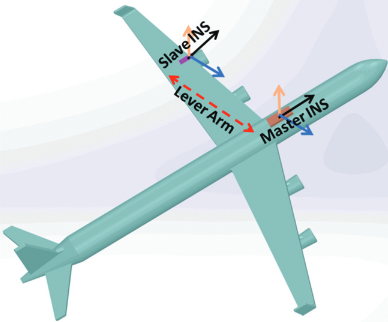
\includegraphics[width=1.0\textwidth]{logos/sambhav1.png}
    \caption{  Location of  Master  INS  and  Slave  INS  in a  typical aircraft-missile configuration (Lever arm).}
    \label{fig:img1}
\end{figure}
\lipsum

\par As shown in Figure 1, in a fighter aircraft Master INS is located at a location where the effect of the lever arm and vibration effect is minimum. Normally this location is along the aircraft axis.

\par Initializing the Slave INS, the Master INS information is communicated to the slave INS with ``nominal lever arm'' compensation as shown in Figure 2. The lever arm vector is the relative distance between the Master INS and the Slave INS. The lever arm compensation is necessary to account for the centripetal and vibration effects when aircraft performs a maneuver during alignment. This one-shot \cite{titterton2004strapdown} transfer of information is used to initialize the slave INS.
\\
\lipsum
\begin{figure}
    \centering
    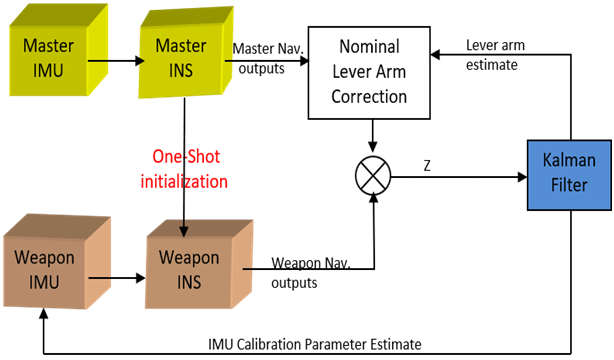
\includegraphics[width=1.0\textwidth]{logos/sambhav2a.png}
    \caption{ Schematic block diagram of transfer alignment scheme.}
    \label{fig:img1}
\end{figure}
\lipsum
\\The measurement of the lever arm is a highly time-intensive process for an aircraft with multiple missile stations. The requirements for the accuracy of measurement of the lever arm increase when the missile is mounted on outbound stations of the aircraft wing. In this paper, the authors tried to align the slave INS without the requirement of lever arm parameters measurement and compensation.
  \end{block}
\end{column}
\separatorcolumn

\begin{column}{\colwidth}

\begin{block}{Navigation Mode}
  
After initialisation of slave INS, the Navigation outputs (PVA) of master INS and slave INS are dynamically compared and errors obtained in the process need to be compensated through Transfer Alignment (TA) for accurate initialization of slave INS. The TA procedure requires aircraft maneuver when both INS are in navigation mode. During the maneuver, the differences in the navigation of both INS are a function of the following errors:
\begin{itemize}
    \item Misalignment errors
    \item Gyro sensor errors
    \item Accelerometer sensor errors
    \item Physical acceleration and rates sensed by slave INS due to rotation-induced acceleration $\omega^2r$ produced by the physical separation (Lever arm).
\end{itemize}

The proposed transfer alignment scheme uses the aircraft take-off maneuver for observability of errors between master and slave INS and does not require any specific maneuver as required in other transfer alignment schemes \cite{dai2019rapid}, \cite{gao2007performance}, \cite{hongzhong2011study}, , \cite{tarrant1993rapid} \cite{xiong2006observability}.

\end{block}

  \begin{block}{Transfer Alignment Formulation}
  
 It involves mainly four steps to perform TA:
 \begin{itemize}
    \item The Kalman Filter
    \item Kalman Recursions
    \item State Transition Matrix $(A_k)$
    \item Misalignment Model
\end{itemize}

\\
\lipsum
\begin{figure}
    \centering
    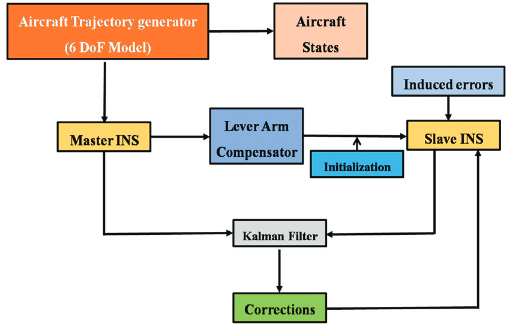
\includegraphics[width=1.0\textwidth]{logos/sambhav3.png}
    \caption{Transfer alignment simulation environment and initialisation flow chart. \cite{reddy2013advanced}}
    \label{fig:img3}
\end{figure}
\lipsum
  \end{block}



\begin{block}{Sensors Specifications}
  
% Table generated by Excel2LaTeX from sheet 'Sheet1'
\begin{table}[htbp]
  \centering
  \caption{Master INS sensor specifications}
    \begin{tabular}{llc}
    \toprule
    \textbf{Parameter} & \textbf{Unit} & \multicolumn{1}{l}{\textbf{Specifications}} \\
    \midrule
    \textbf{Gyro:} &       &  \\
    \midrule
    Bias Stability & Deg/Hr & 0.01 \\
    Input range & Deg/sec & $\pm$ 300 \\
    Scale factor stability & ppm   & 10 \\
    Random walk & Deg/$\sqrt(Hr) & 0.003 \\
    \midrule
    \textbf{Accelerometer:} &       &  \\
    \midrule
    Dynamic range & `g'   & 50 \\
    Bias stability & \mu g & 30 \\
    Scale factor stability & ppm   & 30 \\
    \bottomrule
    \end{tabular}%
  \label{tab:addlabel}%
\end{table}%


% Table generated by Excel2LaTeX from sheet 'Sheet1'
\begin{table}[htbp]
  \centering
  \caption{Slave INS sensor specifications}
    \begin{tabular}{llc}
    \textbf{Parameter} & \textbf{Unit} & \multicolumn{1}{l}{\textbf{Specifications}} \\
    \midrule
    \textbf{Gyro:} &       &  \\
    \midrule
    Bias Stability & Deg/Hr & 5 to 15 \\
    Input range & Deg/sec & $\pm$ 300 \\
    Scale factor stability & ppm   & 100 \\
    Random walk & Deg/ $\sqrt(Hr)$ & 0.03 \\
    \midrule
    \textbf{Accelerometer:} &       &  \\
    \midrule
    Dynamic range & `g'   & 50 \\
    Bias stability & \mu g & 1 \\
    Scale factor stability & ppm   & 50 \\
    \bottomrule
    \end{tabular}%
  \label{tab:addlabel}%
\end{table}%

\end{block}

  
   \begin{alertblock}{Important Point}
    \centering

    \textbf{Scan QR code for Research Paper}

 
 \begin{figure}[h]
    \centering
    
\includegraphics[width = 0.3\textwidth]{logos/paperQR.png}
    \label{fig:my_zero}
\end{figure}
 
 \\ \newline

  \end{alertblock}

\end{column}

\separatorcolumn

\begin{column}{\colwidth}
  \begin{block}{Simulation Environment}
  
The following assumption was considered for simulating the proposed scheme:
\begin{itemize}
    \item A complete error model is required to design an optimal Kalman filter. There are many environmental error sources that cannot be modeled as mathematical models. Hence, a sub-optimal filter is used by simplifying the state dynamics by neglecting certain states.
    \item No specific maneuver requirement, the scheme uses natural maneuvers sensed during the aircraft take-off.
\end{itemize}




  \end{block}

  \begin{block}{Simulation Results}
  
It is considered to bring out the robustness of the algorithm. \\
Case 1: Misalignment of -1, -1, and -1 deg is given between roll, pitch, and yaw axes of Master and Slave INS. \\
Case 2: Misalignment of -5, -5, and -5 deg is given between roll, pitch, and yaw axes of Master and Slave INS.
To evaluate the algorithm, natural pitch and yaw maneuvers experienced by Master and Slave INS during take-off were provided. The roll and pitch angles are estimated immediately and accurately as expected, whereas yaw angle estimation is less accurate. Table 3. Misalignment error (ME) for -1 deg and -5 deg misalignment
% Table generated by Excel2LaTeX from sheet 'Sheet1'
\begin{table}[htbp]
  \centering
  \caption{Misalignment error (ME) for -1 deg and -5 deg misalignment}
    \begin{tabular}{lccccc}
    \toprule
          & \textbf{Yaw ME } &       & \textbf{Pitch ME} &       & \textbf{Roll ME} \\
    \midrule
          & \multicolumn{5}{c}{(mrad)} \\
    \midrule
    \textbf{Case 1} & 0.96  &       & 0.35  &       & 0.49 \\
    \textbf{Case 2} & 1.15  &       & 0.6   &       & 0.8 \\
    \bottomrule
    \end{tabular}%
  \label{tab:addlabel}%
\end{table}%



  \end{block}
  

\begin{block}{Conclusions}
\begin{itemize}
    \item The main objectives   of   the   proposed   scheme   are demonstrated  for  estimating  the  accurate  misalignment between Master and Slave INS and initializing the Slave INS with corrected Position, Velocity, and Attitude from Master INS.
    \item An innovative provision without the need for specific maneuver and lever  arm  compensation,  the  accurate transfer  of  INS  information  demonstrated,  which  avoids the  need  for  extra  maneuver  on  combat  operation  by Aircraft pilot.
\end{itemize}

\end{block}
    \begin{block}{Acknowledgments}
    
The authors are extremely grateful to Dr. J Umakant, Mr. M. Kannan, Mr. R S Chandrasekhar and Mr. Sandeep Pal for sharing their knowledge, valuables ideas, and guidance which are immensely helpful in various stages of this work. The authors also like to express their deep sense of gratitude to Director DRDL, Director RCI, and Dean & Director IIIT Nagpur for giving motivation and opportunity to work on this problem.

\end{block}

\begin{block}{References}

\bibliographystyle{plain}
\bibliography{poster}

\end{block}
\end{column}

\separatorcolumn
\end{columns}
\end{frame}

\end{document}
